\section{Firefox OS}
\label{sec:firefoxOS}

\subsection{Overview}

As said before
Firefox OS is the open-source operating system targeting mobile devices being
developed by Mozilla and based on Web technologies. All the apps in Firefox OS
are Web pages since they are build using only Web technologies and, except when
some special Javascript API are required, can be used in a Web browser.
To create a app from a previous Web page you only need a manifest
file that store some metadatas about the app and a figure to be the icon. The
files
\href{http://fred-wang.github.io/MathUI2014/demos/app/manifest.webapp}{demos/app/manifest.webapp}
and
\href{http://fred-wang.github.io/MathUI2014/demos/app/icon.png}{demos/app/icon.png},
respectively a manifest and a icon,
show the extra files need to create a app for
\href{http://fred-wang.github.io/MathUI2014/demos/app/index.html}{demos/app/index.html}.

Although the Web was initially created to share knowledge, today it is also used
as a platform to create knowledge (e.g. Wikipedia) and in a near future
significant part of the content created in the Web will be done using mobile
devices. For science, technology, engineering and mathematics there is a lack of
tools to deal with math that need to be fill by a ``Math Suite''.

In the next section we give more details about the ``Math Suite'' and
after that we present some of the demos wrote by Mozilla MathML community.

\subsection{Math Suite}

Like an office suite is a collection of softwares intended to be used by
knowledge workers an Math Suite is a collection of softwares intended to be used
by someone that make intensive use of math. The basic components of an Math
Suite is a text processor with math support and an symbolic math programming
language, like Mathematica, but the suite could also have:
\begin{itemize}
  \item searching engines for math expressions;
  \item WYSIWYG math editor;
  \item markup converters (e.g. (La)TeX to MathML and MathML to (La)TeX);
  \item handwriting recognition;
  \item 2D drawing tool that help with, for example,
    \href{http://fred-wang.github.io/MathUI2014/demos/2-mathml-in-svg.svg}{demos/2-mathml-in-svg.svg};
  \item 3D drawing tool that help with, for example,
    \href{http://fred-wang.github.io/MathUI2014/demos/6-mathml-in-webgl.html}{demos/6-mathml-in-webgl.html};
  \item scripting tool that help with, for example,
    \href{http://fred-wang.github.io/MathUI2014/demos/3-mathml-javascript.html}{demos/3-mathml-javascript.html};
  \item accessibility to users with disabilities;
  \item and more.
\end{itemize}

Many of the applications in an Math Suite or not share a set of functions, for
example the searching engine can be used by a text processor and by a ebook
reader, and have
this functions available in a open source Javascript library will make easy to
develop new Web applications that can be customized into standalone applications
to run in desktop and mobile devices.

\begin{figure}[!htb]
  \centering
  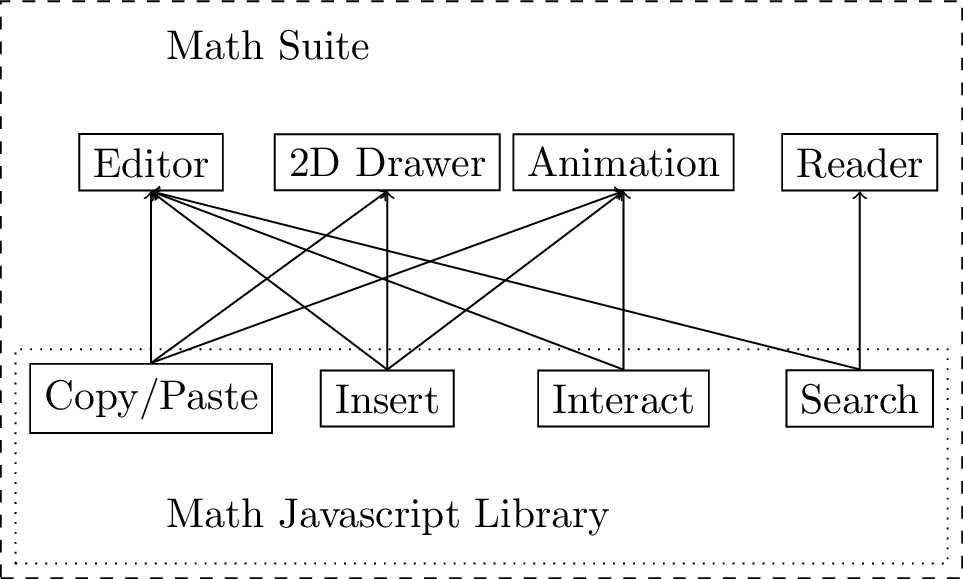
\includegraphics[width=.5\textwidth]{math-suite-diagram.png} \\
  Figure: Illustration of Math Suite.
\end{figure}

The authors of this work start writing this Javascript library as small
independent libraries and some demos that use it.

\subsection{Math Cheat Sheet}

This is a basic app with a collection of common K-12 equations available at
\href{http://r-gaia-cs.github.io/math-cheat-sheet/}{http://r-gaia-cs.github.io/math-cheat-sheet/}.
The equations are organized in sections and a table of contents is provided to
help jumping from one section to another.

Although be a basic app, to build it was necessary a (La)TeX to MathML
conversion (we use TeXZilla) and is a nice way to show that Firefox OS supports
MathML. Only the unstable version of Firefox OS support copy and paste but when
using this app at Firefox with MathML Copy add-on is possible to
copy and paste the MathML and (La)TeX representation of the equations.

Others nice features that can be add to this app in the
future include:
\begin{itemize}
  \item link to resource like Wikipedia related to the equation,
  \item search bar to quickly find the desired equation,
  \item customization of equations, \ldots
\end{itemize}

\subsection{TeXZilla App}

This is a note-taking app for math available at
\href{http://r-gaia-cs.github.io/TeXZilla-webapp/}{http://r-gaia-cs.github.io/TeXZilla-webapp/}.
It takes as input (La)TeX expression, shows a preview of it refreshed during
input and enable the user to save it.

The conversion from (La)TeX to MathML is performed by TeXZilla, introduced at
previous chapter, and no internet connection is required. The save functionality
use IndexedDB, ``an API for client-side storage of significant amounts of
structured data and for high performance searches on this data using indexes''
as explained at Mozilla Developer Network, there is a W3C Candidate
Recommendation.

This app also have some buttons to help the user entry (La)TeX commands like
{\tt \textbackslash frac} and {\tt \textbackslash sqrt}. Right now the buttons
only cover a few commands since the best solution is that the mobile devices
have a virtual keyboard developed with the focus in math (we have plans to build
such keyboard to Firefox OS) and desktop users can rely in a similar keyboard
make available as a add-on.
